\section{Induktives Laden}
Um den Energiespeicher des Dojos aufladen zu können, wird eine induktive Ladeschaltung eingebaut, was Ziel 4 entspricht. In einer externen Ladevorrichtung wird die Netzspannung umgewandelt und auf eine Spule gegeben. Diese Spule erzeugt somit ein magnetisches Feld. Ist der Dojo in Reichweite zu dieser Apparatur und somit im induzierten Energiefeld, wird die Energie von diesem in elektromagnetischer Form in den Dojo transportiert und dort umgewandelt. In der Spule, die sich im Dojo befindet, wird so eine Wechselspannung induziert. Um diese Spannung für die Akkuladung nutzbar zu machen, wird diese mithilfe eines Gleichrichters angepasst und anschliessend noch geglättet. Einen Überblick über die Grobstruktur der Komponenten für die induktive Ladung, gibt Abbildung \ref{fig:Grobstruktur_ind_Laden}. Der Vorteil der induktiven Lademethode besteht darin, dass ein komplett geschlossenes Gehäuse verwenden werden kann und dadurch der Dojo vor eindringender Feuchtigkeit oder Schmutz geschützt ist. Dies wirkt sich auch positiv auf seine Lebenszeit aus. Des weiteren können aufgrund fehlender Anschlüsse auch keine Abnutzungserscheinungen auftreten, welche durch häufiges ein- und ausstecken auftreten können.

\begin{figure}[H]
\begin{center}
	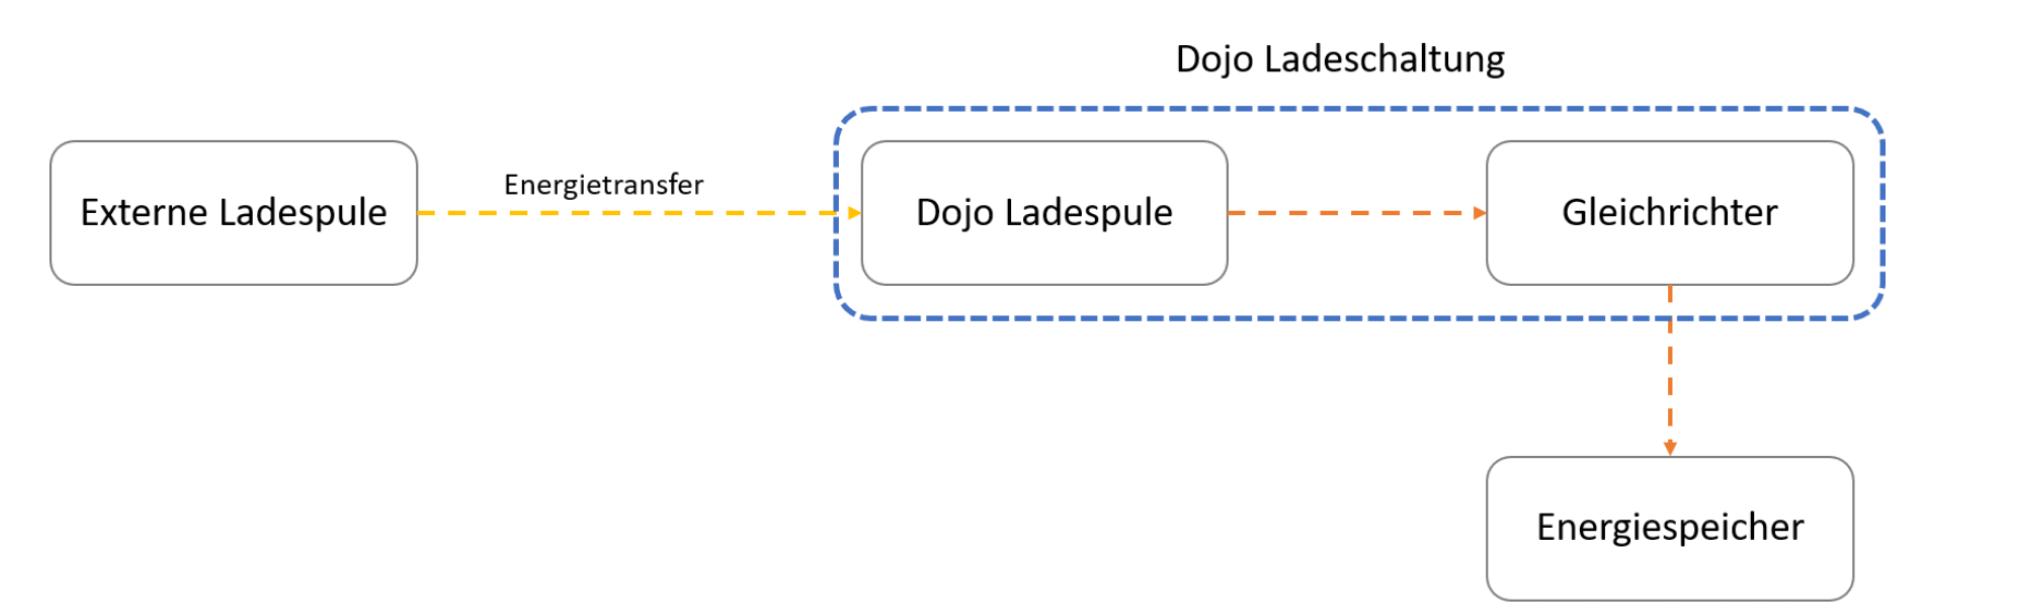
\includegraphics[width=160mm]{data/Induktion.png}
	\caption{Grobstruktur induktives Laden} %picture caption
	\label{fig:Grobstruktur_ind_Laden}
\end{center}
\end{figure}